\documentclass[aspectratio=169]{beamer}

\mode<presentation> {
	\usetheme{Madrid}
	\setbeamertemplate{navigation symbols}{}
}

% ---------- 页尾 ----------
\setbeamertemplate{footline}{
	\begin{beamercolorbox}[wd=\paperwidth,ht=2.5ex,dp=1.25ex]{footline}
		\usebeamerfont{footline}\hspace{0.2cm}\insertshortinstitute%
		\hfill\insertshorttitle\hfill%
		\insertframenumber/\inserttotalframenumber\hspace{0.2cm}%
	\end{beamercolorbox}
}
\setbeamercolor{footline}{fg=orchiddark,bg=orchidlight!30}

% ---------- 二月兰紫配色 ----------
\definecolor{orchidpurple}{RGB}{146,39,143}
\definecolor{orchiddark}{RGB}{115,30,112}
\definecolor{orchidlight}{RGB}{230,210,230}
\definecolor{orchidteal}{RGB}{0,128,128}
\definecolor{orchidteallight}{RGB}{214,235,235}
\definecolor{orchidgold}{RGB}{198,140,0}
\definecolor{orchidgoldlight}{RGB}{250,240,216}

\setbeamercolor{structure}{fg=orchidpurple}
\setbeamercolor{palette primary}{fg=white,bg=orchidpurple}
\setbeamercolor{palette secondary}{fg=white,bg=orchiddark}
\setbeamercolor{palette tertiary}{fg=white,bg=orchidpurple}
\setbeamercolor{palette quaternary}{fg=white,bg=orchiddark}
\setbeamercolor{titlelike}{fg=white,bg=orchidpurple}
\setbeamercolor{frametitle}{fg=white,bg=orchidpurple}
\setbeamercolor{block title}{fg=white,bg=orchidpurple}
\setbeamercolor{block body}{fg=black,bg=orchidlight!22}
\setbeamercolor{item}{fg=orchidpurple}
\setbeamercolor{section in toc}{fg=orchiddark}
\setbeamercolor{block title alerted}{fg=white,bg=orchidteal}
\setbeamercolor{block body alerted}{fg=black,bg=orchidteallight}
\setbeamercolor{block title example}{fg=white,bg=orchidgold}
\setbeamercolor{block body example}{fg=black,bg=orchidgoldlight}
\setbeamercolor{think}{fg=orchiddark,bg=orchidlight!22}

% ---------- 章节过渡页 ----------
\AtBeginSection[]
{
	\begin{frame}
		\centering
		\vspace{1.5cm}
		{\usebeamerfont{title}\color{orchiddark}\insertsectionnumber.~\insertsectionhead}\\
		\vspace{0.5cm}
		{\color{orchidpurple}\rule{0.35\textwidth}{1.2pt}}
	\end{frame}
}

% ---------- 轻量想法/评注框 ----------
\setbeamercolor{think}{fg=orchiddark,bg=orchidlight!22}
\setbeamercolor{thinkg}{fg=orchiddark,bg=orchidgoldlight}
\newcommand{\remark}[2]{%
	\vspace{0.12cm}%
	\begin{beamercolorbox}[rounded=true,sep=6pt]{think}%
		{\color{orchidpurple}\textbf{#1}：}~#2%
	\end{beamercolorbox}%
}
\newcommand{\remarkg}[2]{%
	\vspace{0.12cm}%
	\begin{beamercolorbox}[rounded=true,sep=6pt]{thinkg}%
		{\color{orchidgold}\textbf{#1}：}~#2%
	\end{beamercolorbox}%
}
\newcommand{\remarkp}[2]{%
	\vspace{0.12cm}%
	{\color{orchidpurple}\textbf{#1}：}~#2\par%
}

\usepackage{graphicx}
\usepackage{booktabs}
\usepackage[UTF8,noindent]{ctexcap}
\usepackage[bookmarks=true]{hyperref}
\usepackage{amsmath,amssymb,bm}
\usepackage{tikz}
\usetikzlibrary{shapes.geometric,arrows,positioning}

% ---------- 快捷命令 ----------
\newcommand{\T}{^{\mathsf{T}}}
\newcommand{\R}{\mathbb{R}}
\newcommand{\mat}[1]{\bm{#1}}
\newcommand{\tbf}[1]{\textbf{#1}}

% ============================================================
%	以下为可修改区：标题 / 作者 / 单位 / 日期
% ============================================================

\title[063组分享]{《波浪能装置输出功率优化设计》赏析}
\author{魏舟}
\institute[南京理工大学]
{
	063组 \\
	\medskip
	\textit{wei\_zhou@njust.edu.cn}
}
\date{2026年8月}

% ============================================================
%	以下为正文示例，请按需替换
% ============================================================



\begin{document}

% ============ 10 分钟版正文：以建模思路为主 ============
% ---------- 标题页 ----------
\begin{frame}
	\begin{center}
		\begin{beamercolorbox}[rounded=true,shadow=true,sep=8pt,center,wd=\textwidth]{title}
			\usebeamerfont{title}\inserttitle
		\end{beamercolorbox}
	\end{center}
	\vspace{0.5cm}
	\begin{columns}[c]
		\column{0.5\textwidth}
		\centering
		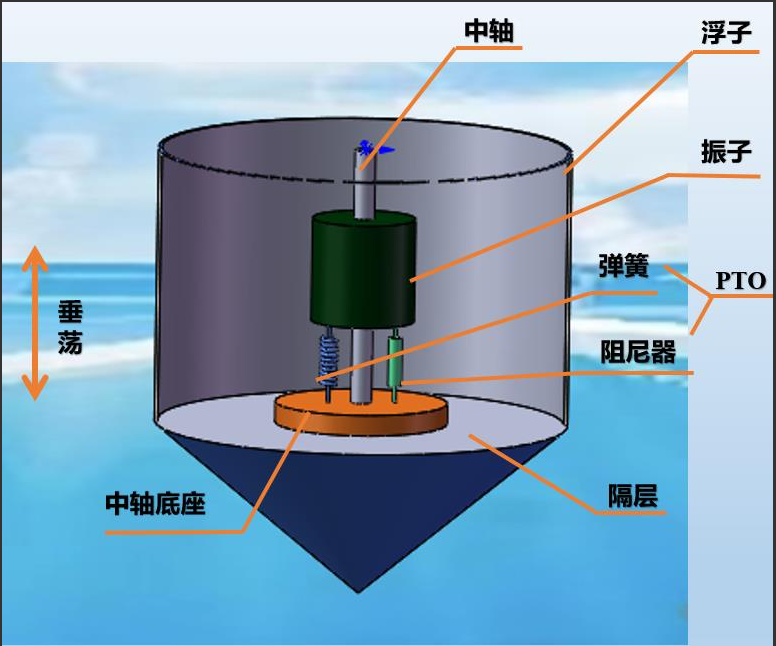
\includegraphics[width=0.9\textwidth]{Figure/波浪能装置示意图.png}

		\column{0.5\textwidth}
		\centering
		{\usebeamerfont{author}\usebeamercolor[fg]{author}\insertauthor}\\[0.4cm]
		{\usebeamerfont{institute}\usebeamercolor[fg]{institute}\insertinstitute}\\[0.4cm]
		{\usebeamerfont{date}\usebeamercolor[fg]{date}\insertdate}
	\end{columns}
\end{frame}

% ---------- 目录 ----------
\section*{目录}
\begin{frame}
	\frametitle{汇报提纲}
	\tableofcontents
\end{frame}
\setcounter{section}{0}

% ---------- 建模思路总览 ----------
\section{建模思路总览}
\begin{frame}
	\frametitle{拿到这道题，思路就六步}
	\scriptsize
	\begin{center}
	\begin{tikzpicture}[
		stepbox/.style={draw=orchidpurple, thick, rounded corners=3pt,
			minimum width=1.75cm, minimum height=1.5cm, align=center,
			fill=orchidlight!35, font=\scriptsize},
		arrow/.style={-stealth, thick, orchidpurple}
	]
		\node[stepbox] (a) at (0,0) {1审题\\把题干翻成\\建模需求};
		\node[stepbox] (b) at (2.35,0) {2物理建模\\受力分析\\列方程};
		\node[stepbox] (c) at (4.7,0) {3数值求解\\转一阶\\龙格库塔};
		\node[stepbox] (d) at (7.05,0) {4目标约束\\平均功率\\阻尼范围};
		\node[stepbox] (e) at (9.4,0) {5寻优\\粗扫+遗传算法};
		\node[stepbox] (f) at (11.75,0) {6检验\\周期+扰动};
		\draw[arrow] (a.east) -- (b.west);
		\draw[arrow] (b.east) -- (c.west);
		\draw[arrow] (c.east) -- (d.west);
		\draw[arrow] (d.east) -- (e.west);
		\draw[arrow] (e.east) -- (f.west);
	\end{tikzpicture}
	\end{center}
	这篇论文最值得学的，不是某个公式，而是这六步一环扣一环的\textbf{建模思路}：每一步都知道自己在哪、要往哪走。
\end{frame}

% ---------- 第一步：审题 ----------
\section{第一步：审题}
\begin{frame}
	\frametitle{审题：怎么把题干翻成建模需求}
	\scriptsize
	\begin{block}{读题干抓三样}
		\begin{itemize}
			\item \textbf{装置结构}：谁在动、怎么动（浮子带振子，PTO 弹簧+阻尼做功）
			\item \textbf{受力来源}：海水给浮子四类力（激励、附加惯性、兴波阻尼、静水恢复）
			\item \textbf{要算什么}：四问递进，建模/优化 $\times$ 单运动/双运动
		\end{itemize}
	\end{block}
	\begin{block}{四类力 $\rightarrow$ 方程里的项}
		激励力 $f\cos\omega t$、附加质量 $m_a$、兴波阻尼 $B_v$、静水恢复 $-\rho g A x$，全都能对应到后面方程的一个项
	\end{block}
	\remark{我的想法}{审题不是把题目念一遍，而是按``建模需要什么''去拆：结构、受力、目标各在哪，心里先有张图。}
\end{frame}

% ---------- 第二步：物理建模 ----------
\section{第二步：物理建模}
\begin{frame}
	\frametitle{物理建模：受力分析 $\rightarrow$ 牛顿第二定律}
	\scriptsize
	\begin{columns}[T]
		\column{0.5\textwidth}
		\begin{block}{先建坐标系，再受力分析}
			\begin{itemize}
				\item \textbf{大地系} $OXYZ$：固定；\textbf{固体系} $oxyz$：随浮子动；$x_r=x_2-x_1$
				\item 浮子受：激励力、附加惯性、兴波阻尼、静水恢复、PTO 作用力；振子受 PTO 反力
			\end{itemize}
		\end{block}
		\begin{center}
			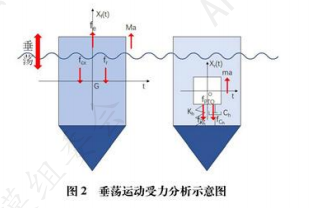
\includegraphics[height=0.3\textheight]{Figure/垂荡运动受力分析示意图.png}\\
			\scriptsize 浮子与振子受力分析（示意）
		\end{center}
		\column{0.5\textwidth}
		\begin{block}{列方程（牛顿第二定律）}
			浮子：$(m_1+m_a)\ddot x_1=f\cos\omega t-B_v\dot x_1-\rho g A x_1+f_d+f_k$\\
			振子：$m_2\ddot x_2=-f_d-f_k$\\
			$f_d=-C(\dot x_1-\dot x_2)$，$f_k=-K(x_1-x_2)$
		\end{block}
		\remark{我的想法}{顺序很重要：先想清楚坐标系和受力，再列方程。跳过这步直接写方程，多半写一半就乱。}
	\end{columns}
\end{frame}

% ---------- 第三步：数值求解 ----------
\section{第三步：数值求解}
\begin{frame}
	\frametitle{数值求解：二阶转一阶 + 四阶龙格库塔}
	\scriptsize
	\begin{block}{为什么要数值解}
		方程是二阶微分方程组，没有闭式解；从初值出发，一个小步长一个数往前递推
	\end{block}
	\begin{block}{怎么递推}
		\begin{itemize}
			\item 二阶转一阶：把 $x,\dot x$ 当状态，问题一是 4 个一阶方程，问题三变 8 个
			\item \textbf{四阶龙格库塔}：一个步长内取起点、中点、终点多个斜率加权
			\item 步长 $10^{-4}$，求前 40 周期，按 0.2s 间隔采样
		\end{itemize}
	\end{block}
	\remark{我的想法}{步长不是随便定的：太大 40 个周期算到后面就抖，太小算不动。$10^{-4}$ 是精度和速度的折中，这个细节我以前不会想。}
\end{frame}

% ---------- 第四步：目标与寻优 ----------
\section{第四步：目标与寻优}
\begin{frame}
	\frametitle{目标与约束：优化模型怎么写}
	\scriptsize
	\begin{block}{目标：平均输出功率}
		$P_{avg}=\dfrac{1}{t_2-t_1}\int_{t_1}^{t_2} C(\dot x_1-\dot x_2)^2\,dt$，只取\textbf{稳态段} $[100,180]$s 求平均
	\end{block}
	\begin{block}{决策量与约束}
		\begin{itemize}
			\item 决策量：直线阻尼系数 $C\in[0,100000]$
			\item 或 $C=\alpha|v_r|^\beta$，$\alpha\in[0,100000]$，$\beta\in[0,1]$
		\end{itemize}
	\end{block}
	\remark{我的想法}{为什么只取稳态段？前面有一段瞬态，功率不稳，取平均会把结果带偏。这个取舍是算平均功率的关键。}
\end{frame}

\begin{frame}
	\frametitle{寻优：梯形积分 + 先粗后精 + 遗传算法}
	\scriptsize
	\begin{block}{怎么算功率积分}
		积分没法解析求，用\textbf{梯形法}把 $P(t)$ 离散成小梯形面积之和，步长越小越准
	\end{block}
	\begin{block}{怎么找最优阻尼}
		\begin{itemize}
			\item \textbf{先粗扫}：大步长遍历阻尼，找到功率峰大致位置
			\item \textbf{遗传算法精找}：迭代 200 代，避免卡在局部最优
		\end{itemize}
	\end{block}
	\begin{block}{结果}
		题2(1) $P_{max}=229.68$W、$C=37639$；题2(2) $P_{max}=230.02$W、$C=81478$
	\end{block}
	\remark{我的想法}{``先粗后精''这套组合看着简单，但比我直接暴力遍历快太多，又能跳出局部最优，以后优化题都这么干。}
\end{frame}

% ---------- 第五步：模型检验 ----------
\section{第五步：模型检验}
\begin{frame}
	\frametitle{检验：用物理常识当标尺}
	\scriptsize
	\begin{block}{验模型对不对}
		受迫振动稳定后\textbf{周期必等于激励周期}，比较响应周期与理论周期的方差 $\delta$：垂荡 $\delta=0.0017,0.0034$，纵摇 $\delta=0.00036$，都极小
	\end{block}
	\begin{block}{验结果稳不稳}
		对转动惯量加 $\pm1\%$ 扰动重算，结果偏差 $<0.1\%$，说明对参数不敏感、求解可靠
	\end{block}
	\remark{我的想法}{以前以为检验必须靠实验数据，这篇告诉我：没有实验也能验——用物理常识当标尺，再给参数加扰动看结果动不动。}
\end{frame}

% ---------- 第六步：多自由度推广 ----------
\section{第六步：多自由度推广}
\begin{frame}
	\frametitle{从垂荡推广到垂荡+纵摇：思路怎么复用}
	\scriptsize
	\begin{block}{加一个自由度的套路}
		\begin{itemize}
			\item 多一组转动惯量（平行移轴、垂直轴定理算）$\rightarrow$ 多一套力矩方程
			\item 求解完全复用：转一阶 + 四阶龙格库塔，状态从 4 个变 8 个
			\item 优化升级为二维：同时求直线阻尼 $C$ 和旋转阻尼 $C_t$
		\end{itemize}
	\end{block}
	\begin{block}{结果}
		问题4 双阻尼优化：$P_{max}=316.58$W，$C=58944$，$C_t=98227$
	\end{block}
	\remark{我的想法}{多自由度的题，其实就是单自由度复制几份再串起来。会一个就差不多会一串，这是这篇最省力的一点。}
\end{frame}

% ---------- 心得与收获 ----------
\section{心得与收获}
\begin{frame}
	\frametitle{心得与收获}
	\scriptsize
	\begin{itemize}
		\item \textbf{审题}：按建模需要拆题干——结构、受力、目标各在哪
		\item \textbf{建模}：先受力分析、再列方程，每一项都能对上受力图
		\item \textbf{方法}：牛顿定律 + 龙格库塔 + 遗传算法，一套打到底
		\item \textbf{优化}：先粗扫再精找，避开局部最优；约束给具体范围
		\item \textbf{检验}：物理常识当标尺（周期吻合），参数扰动验可靠性
	\end{itemize}
	\remark{我的收获}{这五点是我读完整篇最想带走的。建模题不怕方法多，怕的是思路乱——六步走稳，比背一堆模型管用。}
\end{frame}

% ---------- 结束页（致谢） ----------
\begin{frame}
	\centering
	\Huge{感谢聆听！}\\[1cm]
	\Large{敬请各位老师、同学批评指正}
\end{frame}

\end{document}
